\documentclass{article}
\usepackage[utf8]{inputenc}
\usepackage[none]{hyphenat}
\usepackage{geometry}
\usepackage{graphicx}
\usepackage{mathtools}
\usepackage{gensymb}
\usepackage{titlesec}

\setcounter{secnumdepth}{4}
\title{Rapport de Laboratoire n\degree4}
\author{Groupe 11.57: Théophile d'Ursel, Robin Lannoy, Ghislain Lieukap\\ Kekouonmi,
Amine Mounzer, Maxime Sion et Guillaume van der Rest}
\date{7 Mars 2019}
\geometry{
 a4paper,
 total={170mm,257mm},
 left=20mm,
 top=20mm,
}

\begin{document}
\maketitle
\section{Objectifs du Labo}
L'objectif de ce laboratoire était d'explorer le fonctionnement des inductances, et plus précisément l'inductance mutuelle
et les courants induits. Notre but était de trouver un moyen d'évaluer l'inductance d'une bobine, sans disposer d'un
inductomètre. Aucune technique ne nous était donnée, il nous fallait donc imaginer un moyen d'évaluer ces deux paramètres.
\section{Connaissances Préliminaires}
Pour imaginer un moyen d'évaluer les deux inductances, plusieurs notions d'électricité sont à maitriser:
\begin{itemize}
    \item La Loi d'Ohm: $V = R\cdot I$
    \item Les formules propres aux inductances en courant alternatif: $V = L \frac{dI}{dt}$, $X_{L} = \omega L$ avec $V$, la tension
    aux bornes de l'inductance, $L$, la valeur de cette inductance, et $\omega$, la vitesse angulaire du courant, exprimée par $\omega = 2\pi f$
    \item Les formules d'inductance mutuelle: $M \overset{\Delta}{=} \frac{N_{2} \Phi_{2,1}}{I_{1}} = \frac{N_{1} \Phi_{1,2}}{I_{2}}$
    \item L'utilisation d'un phaseur, et la formule de l'impédance d'un circuit LR à tension alternative:
    \newline
    $I(t) = \frac{V_{s}cos(\omega t)}{\sqrt{R^{2} + X_{L}^{2}}}$
    \item L'utilisation d'un oscilloscope, d'un générateur de fréquence, et d'un multimètre.
\end{itemize}
\section{Mode Opératoire et Prédictions théoriques}
\subsection{Matériel à disposition}
\begin{itemize}
    \item Résistances de 10 k$\Omega$
    \item \textit{Breadboard} \textbf{\textit{WISH}}
    \item Cables de tailles diverses
    \item Oscilloscope \textit{\textbf{METRIX OX530}}
    \item Générateur de signaux \textit{\textbf{Topward 8120}}
    \item Inductances de 27 $\mu H$
\end{itemize}
\newpage
\subsection{Circuits à Réaliser et Résultats théoriques}
\subsubsection{Premier Circuit: Inductance propre}
\begin{figure}[h]
    \centering
        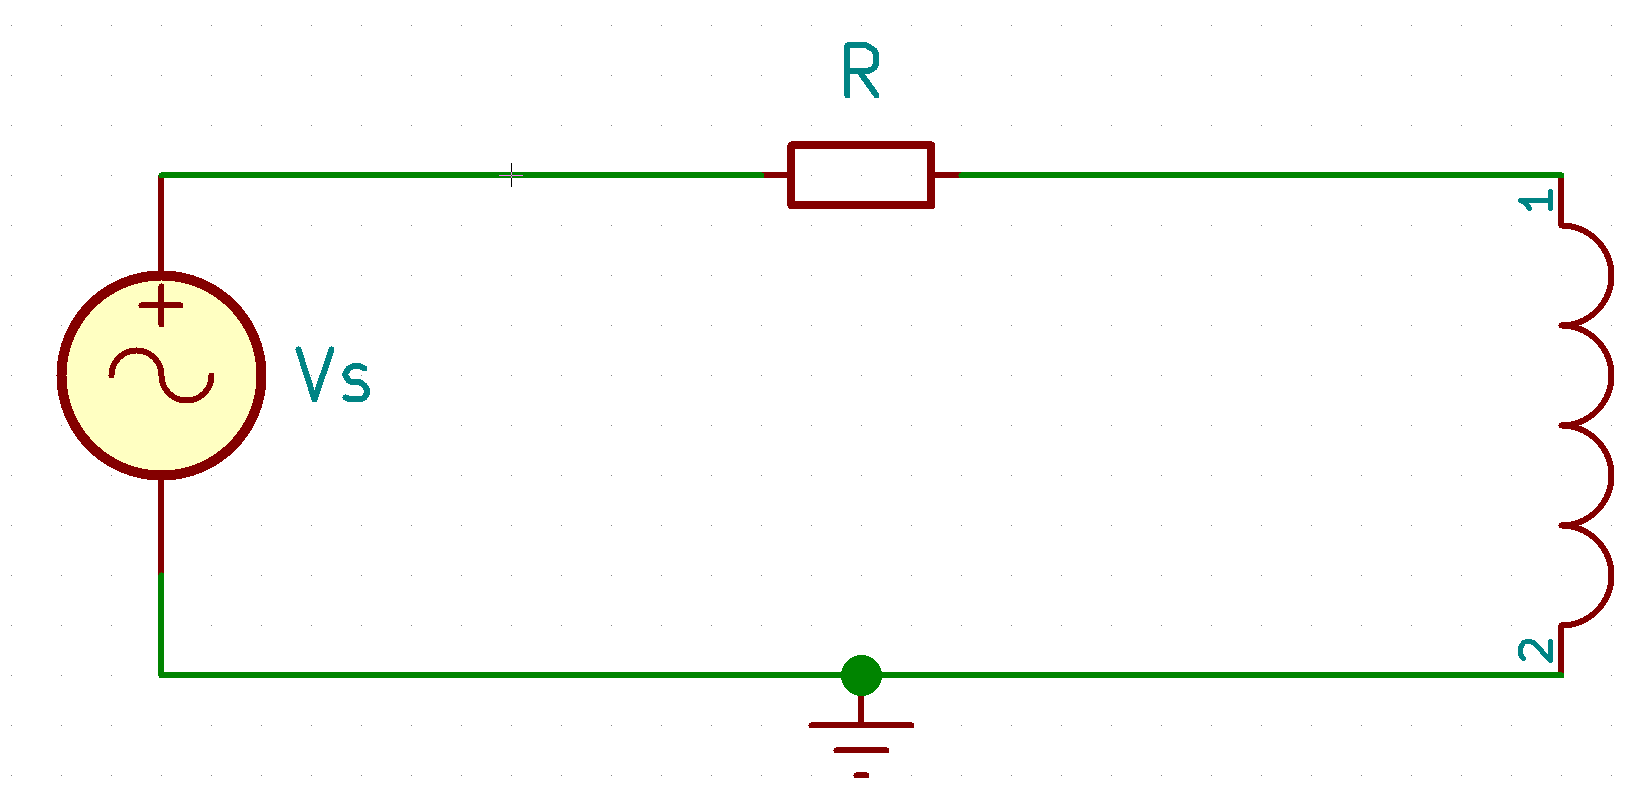
\includegraphics[scale = 0.12]{LR.png}
        \caption{Schéma d'un montage servant à déterminer une inductance}
        \label{fig:my_label}
    \end{figure}
Ce circuit nous permet d'évaluer la valeur de l'inductance L. Nous pouvons dire que le courant dans l'inductance vaut
$I(t) = \frac{V_{s}cos(\omega t)}{\sqrt{R^{2} + X_{L}^{2}}}$. Afin de mesurer ce courant, nous mesurons la tension aux
bornes de la résistance et en utilisant la loi d'Ohm nous pouvons déterminer $I$. A partir de cette valeur (maximale) de
$I$, nous déterminons la valeur de $L$ par la relation 
\begin{equation}
    L = \frac{\sqrt{\frac{V_{s}}{I}^2 - R^2}}{\omega}
\end{equation}
\subsubsection{Deuxième Circuit: Inductance Mutuelle}
\begin{figure}[h]
    \centering
        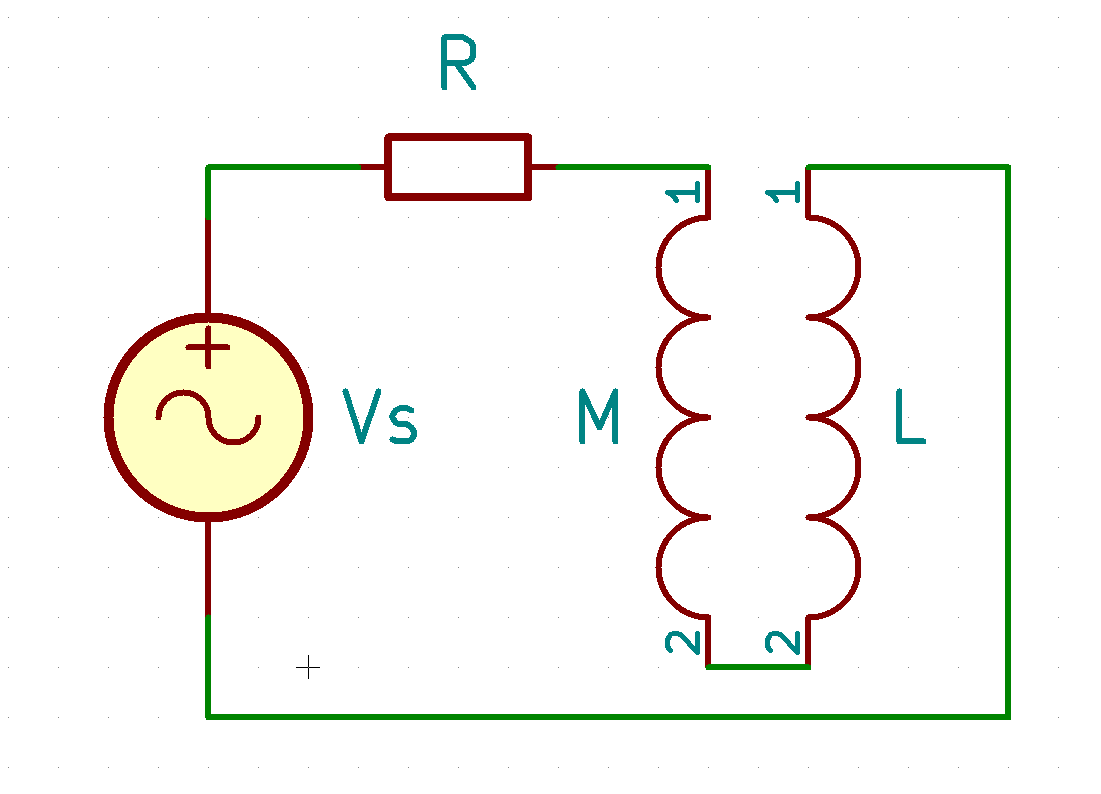
\includegraphics[scale = 0.12]{RM.png}
        \caption{Schéma d'un montage servant à déterminer l'inductance mutuelle}
        \label{fig:my_label}
    \end{figure}
Ce circuit nous permet de déterminer la valeur de l'inductance mutuelle $M$.
Nous pouvons donc déterminer, en connaissant $L_{1}$ et $L_{2}$, que nous venons de mesurer, la valeur de $M$.
Dans ce circuit, nous avons que $V_{s} = V_{L} + V_{R}$. Nous avons aussi $V_{R} = I\cdot R$. En utilisant les formules
phaseur-complexe, nous avons que $V_{L_{1}} = L_{1}\omega I_{1}j - M\omega I_{1}j$ et 
$V_{L_{2}} = L_{2}\omega I_{2}j - M\omega I_{2}j$ ainsi que $I_{1} = I_{2}$. Cela nous donne la relation
\begin{equation}
    V_{s} = (R + L_{1} + L_{2} - 2M)\cdot V_{R}R
\end{equation}
\section{Déroulement du Laboratoire et Résultats}
\subsection{Circuit 1}
La réalisation du circuit était évidemment aisée, et de même pour la prise des mesures. Nous avons mesuré une 
tension  de 5 Volts aux bornes de la résistance, avec une alimentation à 100 kHz, ce qui nous a beaucoup étonnés, et en utilisant l'équation (1)
nous avons une inductance de 0.
il est facile de voir qu'utiliser une résistance de 10 k$\Omega$ ne permet pas d'être très précis. Nous avons réessayé avec
une résistance de 10 $\Omega$ et une fréquence de 100 Khz. Nous avons alors mesuré une tension de 2.5 V aux bornes
de la résistance. Cela nous indique un courant de 0.25 A, nous donnant par l'équation (1) une inductance de 27.56 $\mu$H

\end{document}